

% [You should answer the question: What is the problem?]

% This paragraph should establish the context of the reported work. To do that, authors discuss over related literature (with citations\todo{How to make citations}\footnote{To cite a work in latex  }) and summarize the knowledge of the author in the investigated problem.

% An introduction should answer (most of) the following questions:
% \begin{itemize}
% 	\item What is the problem that I want to solve?
% 	\item Why is it a relevant question?
% 	\item What is known before the study?
% 	\item How can the study improve the current solutions?
% \end{itemize}

% To write it, use if possible active voice:
% \begin{itemize}
% 	\item I are going to watch a film tonight (Active voice).
% 	\item A film is going to be watched by us tonight (Passive voice).
% \end{itemize}
% The use of the first person is accepted.

\chapter{Introduction}
Since the advancement of robotics in the modern society with robots' reliability and high work quality, robots are being used together as a multi-robot system, providing advantage compared to a single robot \cite{Eijyne2020DevelopmentOA}. 
Multi-robot systems are widely employed in various applications such as healthcare facilities to assist elderly residents \cite{retire2017}, industrial plant inspection\cite{Chun12}.
Thinking of an office building where people have different working schedules. If at least one person is in the office, the office is considered occupied. The robot working at this office environment should not only interact with people but also to avoid waste energy by moving to empty rooms. This requires the robots to learn from the office environment information and schedule their activities accordingly. 

For a working robot, environment information is indispensable for efficiently perform activities. There are several types of environment information: (1) Information about its surrounding, such as the position of furniture, doors, walls, and other robots. (2) Information about room occupation which presents the probability of finding a person in the room. The latter may change during long-time operating. Therefore, the long-term room occupation measuring should be conducted to keep its value up to date.
However, current sensing technology, especially for the case of robots equipped with external sensors, is not good enough to gather room occupation information of all rooms satisfactorily. 
Although the camera is able to identify whether there is someone in the office, it is susceptible to changes in lighting conditions and the appearance of objects. Moreover, the field of view is too narrow. Besides, if I install sensors on robots, the vibrations of a robot body can cause damage to the sensors or incorrect measurement results \cite{PYO2015148}. Especially, sensors on robot are not able to capture the background changes, which can cause an incomplete measurement result table.

Therefore, I have considered fixed sensors in the office environment. The fixed sensors are not only stable but also can accurately perform long-term environmental measurements. In order to perform long-term measurement, the sensors use low-power and wireless communication technology and without connected to the centralized pool. To be more precise, its measurement results are stored in its local memory and acquired by the passing robots. In addition, to keep the room occupation information in the multi-robot system and in the sensors synchronized, the centralized pool may assign the robot to some unsynchronized sensors to gather information.

I have developed a multi-robot system able to share the information among sensors, charging stations, robots and the centralized pool. The robot can start five kinds of interactions: 
(1) As long as the robot enters the range of the sensor, they conduct a rapid exchange of room occupation information. 
(2) The robot interacts with a charging station at the beginning and at the end of charging process. 
(3) When the robot is idle, it autonomously requests a task from the centralized pool. The centralized pool then responds robot with a command of a simple task (task contains one target position) or a complex task (task which can be decomposed into multiple simple tasks). This command contains the when and where to perform activity(s). These activities include ``execute task'', ``charging'',``gather information'' etc. (Figure \ref{fig:system_architecture}).
(4) While performing activities, the robot sends acquired room occupation data to the centralized pool. 
(5) Once the robot finished all activities, the robot notifies the central pool that the task is succeeded and idle state again.


I also have implemented a multi-robot task scheduling architecture in the centralized pool. The goal of multi-robot task scheduling is to find the optimal task for the robot in order to minimize the total cost. According to the application requirements, three cost function are designed to calculate cost for ``gather information task'', ``execute task'' and ``charging task''. The cost consider decision variable such as energy consumption, time, room occupation, priority etc. 


I also pay particular attention to error handling to robust against robot failures. 
Two failure cases are considered here. First, sometimes the robot may not able to handle the assigned task within a fixed deadline, since the target position is temporarily unreachable (e.g. blocked by a closed door). In this case, the blocked robot sends failure detail to the centralized pool and request another task. The failed task will then be processed and reused for task scheduling. Second, sometimes the robot may have low battery level, but it fails recharging since all charging station are occupied or the charging station does not respond to the robot. In this case, the deficient robot sends failure detail to the centralized pool. This failure will then be observed by the user and the deficient robot waits for the user to manually control it \cite{Shah7}.

In addition to the architecture I proposed herein, our system uses existing platform called Robot Operating System (ROS \cite{ROSWEB}) to archive core autonomous robot function (navigation, localization, and mapping). Thanks to the ROS, I was able to develop a flexible and efficient system. Adding or removing modules including robots, sensors or charging station is simple and straightforward \cite{Shah7}.

%Finally, I have conducted the systematic experimental evaluation of my design and implementation. I have found out not only which decision variables are necessary for task scheduling but also the relative weight for each decision variable. I have also 


%the centralized pool are responsible for plan and facilitate tasks to the robots according to environment information while the robot decomposes the task into activities and performs them sequencially. 
%Based on the above requirements, 
%The robot and the central pool not only exchange aquired room occupation information, but also exchange task status.
%The centralized pool considers all information and always providing the optimal tasks to robots. 
%If the office building uses a large amount of robots, each of them need to plan an efficent route through the offices without colliding with other robots, without take the same task others are executing and without gather environment information in the same office. Therefore, 
%balance gather environment information and perform task.

%I also have been developing a communication protocal between robot and sensor, and between robot and centralized pool.

\section{Motivation}
%A good introduction usually starts presenting a general view of the topic and continues focusing on the problem studied. Begin it clarifying the subject area of interest and establishing the context (remember to support it with related bibliography).
Given an office building where people have different working schedules. If at least one person is in the office, the office is considered occupied.
When multiple robot working in this environment, an efficient task scheduling algorithm is required, in order to minimize the completion time while decreasing the total power consumption \cite{Chun12}.
In this case, room occupation becomes a valuable decision variables for task scheduling, which describes the possibility that the robot can enter the office.
%However, the sensors attached to robot are typically highly not able to measure room occupation, because the vibrations of a robot body can cause damage to the sensors or incorrect measurement results.
Although there are increasing amounts of research have been conducted in the area of task scheduling for multi-robot system \cite{Shah7}, unfortunately, current research work mainly on multi-robot cooperation dynamic environments and rarely address on adoption of Internet of Things technologies. 
Therefore, I consider adding more fixed sensors to in the whole office environment \cite{Coltin10}, and implement a multi-robot system. This multi-robot system should be able to acquire the room occupation information, and use it as one of decision variables to schedule tasks. 





%run for a long time without changing batteries frequently is a challenge. 




%To solverobot should exploit room occupation information coming from sensors embedded in the environment.


%I have developed a multi-robot system, in which the robot exploit room occupation information coming from sensors embedded in the environment, and the centralized scheduler utilize the room occupation information together with other evaluation parameters (e.g. battery consumption) to plan and facilitate tasks. 


%On the other hand, the sensors attached to robot are typically highly limited. Because the vibrations of a robot body can cause damage to the sensors or incorrect measurement results.

%Moreover, I have implemented the multi-robot system to utilize room occupation as well as common factors (e.g. priority, battery consumption etc.) to schedule tasks. 

%they didn't utilize room occupation information to schedule the tasks. 
%The room occupation shows the possibility that the robot can enter the office. 

\section{Problem definition}
%Additionally, focuses the text on the relevant points of your investigation and problems that you want to solve, relating them with the first part.
In order to develop a multi-robot system, first I need to set up some working environment as well as the assumptions within the environment \cite{Shah7}. The environment is shown in Figure \ref{fig:room_division}, which contains a corridor along the central x-axis and 16 rooms located around the corridor. There is no robot limitation in these rooms, as long as the door of the room is opened, it can be entered by any robot. In addition, there are charging stations in the corridor to charge the robots (Figure \ref{fig:positions_door_station}). Each room has one or multiple doors and each door is attached with a sensor. It is assumed that the people have different working schedule, which cause the room occupied and unoccupied regularly.
Consider that there are a set of robots and a set of different tasks randomly distributed in different rooms. 
Here robot is responsible for moving in 2-dimensional physical space as well as gathering measurement result from sensors. It has a rechargeable battery, and its level drops as robot moves and rotates.
The task requires one robot to traverse a path in the workspace and carry out certain activities, such as gather information, charging or transportation \cite{Ivan2017}. The tasks are classified into two types: simple task (task contains one target position) and complex task (task which can be decomposed into multiple simple tasks). It is assumed that the robot can localize itself within the office environment. The robots are expected to move to the positions where the tasks are located and complete the tasks. 

I split the problem into three sub-problems:
\begin{enumerate}
    \item The first problem is the task scheduling problem. An efficient centralized task scheduling algorithm should be implemented for multi-robot system using the knowledge of room occupation, in order to complete all tasks as soon as possible. 
    \item The second problem is the gather information problem, in which the robots are scheduled to gather room occupation information from fixed sensors, in order to keep room occupation information up to date.
    \item The third problem is the communication problem, an efficient communication protocol should be developed to allow share the information between components in multi-robot system.
\end{enumerate}

%the system environment is an office environment. The SLAM (Simultaneous Localization and Mapping) is a technique to draw a map by estimating current location in an arbitrary space \cite{T3SLAM}. Map (Figure \ref{fig:room_division}) is created by SLAM.

\begin{figure}[htbp]
	\centering
	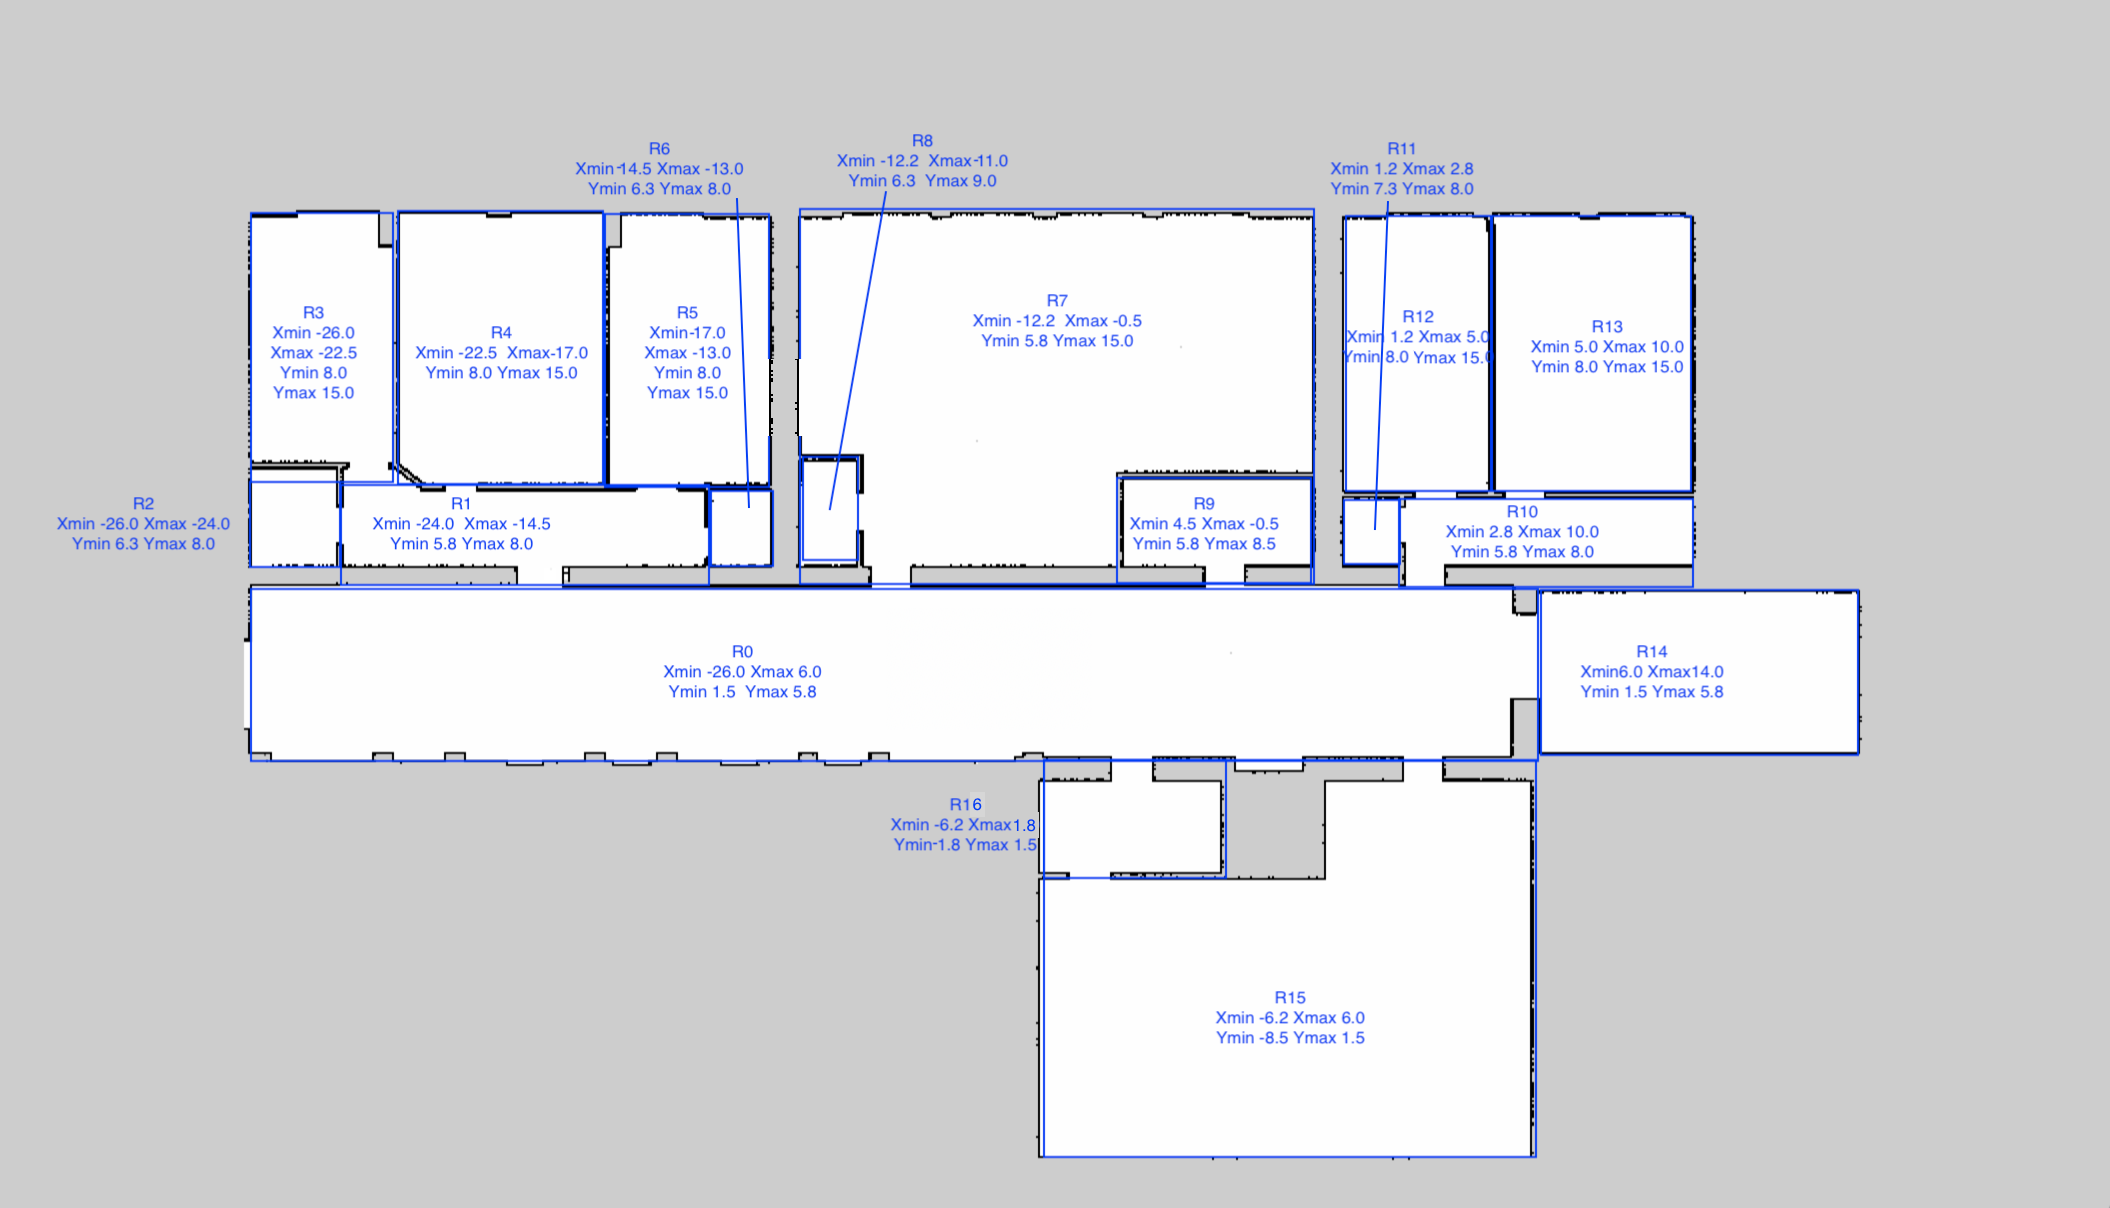
\includegraphics[width = 0.9\textwidth]{content/images/ch3/room_division.png}
	\caption{Room division. The environment is divided into regions that represent rooms in the facility (Figure \ref{fig:room_division}). If the coordinate of a point is in a region, it can be judged that the point is located in the corresponding room.}
    \label{fig:room_division}
\end{figure}

\begin{figure}[htbp]
	\centering
	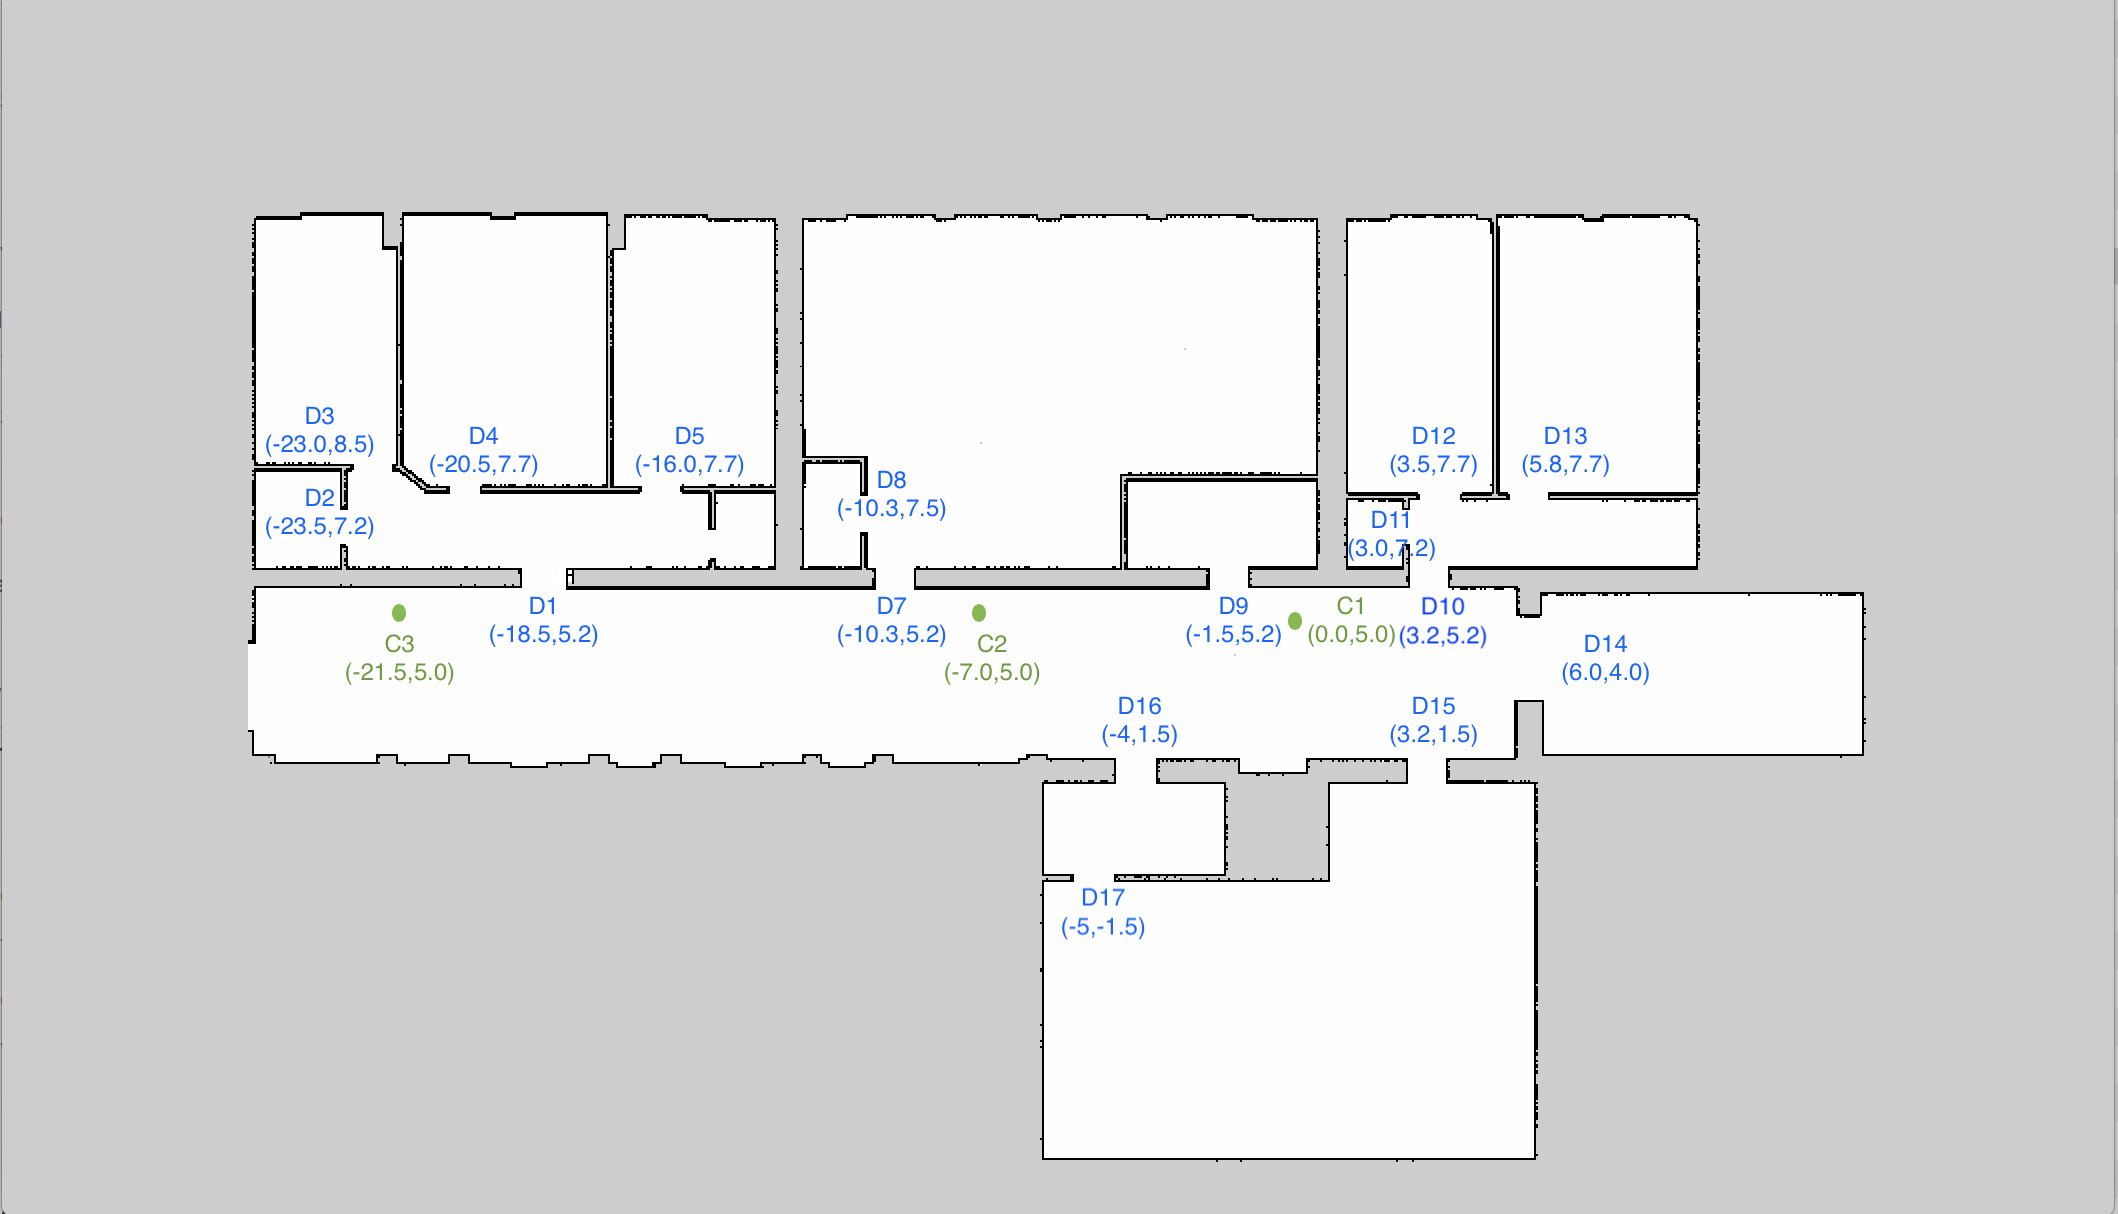
\includegraphics[width = 0.9\textwidth]{content/images/ch3/positions_door_station.png}
	\caption{Positions of Charging Stations (C1-C3) and Doors (D1-D17)}
    \label{fig:positions_door_station}
    \begin{itemize}
        \item \textbf{Doors.} The positions of doors (Figure \ref{fig:positions_door_station}) are stored in database. There are used by a ROS door simulator node, which broadcasts positions and door status periodically. The broadcast messages are received and filtered by robots.
        \item \textbf{Charging Stations.} The positions of charging stations (Figure \ref{fig:positions_door_station}) are used by ROS charging station nodes. For details please refer to Chapter \ref{sec:charging_station}.
    \end{itemize}
\end{figure}


\section{Thesis Structure}
%Present your work to the reader giving a brief overview of what is going to cover every chapter. Write only general concepts, no more than one or two sentences per chapter should be necessary. 
Next chapter briefly introduces the background information and the relative work in both task scheduling and cost function.
In chapter 3 I formally present the architecture of the multi-robot system as well as the approaches to schedule tasks. 
In chapter 4 I describe the implementation of communication protocol and components in the multi-robot system.
Chapter 5 introduces the experiments performed on the implementation. 
Finally, in chapter 6 I interpret the results of the performed work.